\graphicspath{{img/ch5}}
\section{Related Unmanned Missions}

The exploration of lunar pits and lava tubes has evolved from observational curiosities to central themes in planetary science and lunar exploration. These structures offer insights into the Moon’s volcanic history, access to subsurface voids, and potential sites for human habitation and resource utilization.

\subsection{Past Missions}

\textbf{Apollo Program:} 
Although not unmanned, the Apollo missions laid the groundwork for lunar exploration. Apollo 15, in particular, revealed the Hadley Rille, a feature interpreted as a collapsed lava tube. The Apollo Lunar Sounder Experiment (ALSE), flown on Apollo 17, provided radar data that hinted at subsurface voids \cite{radar-observations-lava-tubes}. Although the technology of the time lacked precision for detailed subsurface exploration, these missions demonstrated the potential of radar techniques for future investigations.

\textbf{SELENE (Kaguya):} 
Japan's SELENE mission, launched in 2007, was pivotal in identifying the Marius Hills Hole (MHH), a skylight into a potential lava tube. Using the Lunar Radar Sounder (LRS), SELENE detected transitions between solid material and hollow voids, providing the first direct evidence of intact lava tubes \cite{cavities-selene-lavatubes}. SELENE also demonstrated the potential for radar sounders to penetrate the lunar surface and reveal hidden subsurface structures.


\cite{lro}

\textbf{Chang’e Missions (China):} 
China’s Chang’e-3 and Chang’e-4 missions utilized ground-penetrating radar (GPR) to investigate subsurface structures. These missions identified cavities beneath the regolith and offered detailed profiles of the subsurface near their landing sites \cite{radar-observations-lava-tubes}. These results marked significant advancements in the use of radar for planetary exploration.

\subsection{Active Missions}

\textbf{Lunar Reconnaissance Orbiter (Ongoing):} 
Since its launch in 2009, NASA's Lunar Reconnaissance Orbiter (LRO) has revolutionized our understanding of the Moon, particularly its subsurface features. Equipped with an advanced suite of instruments, the LRO has enabled high-resolution mapping, identification of critical features, and assessment of resources essential for future lunar exploration.

\textbf{Key Highlights:}
\begin{itemize}
    \item The \textbf{Narrow Angle Camera (NAC)} has identified over 300 lunar pits, including the Mare Tranquillitatis pit \cite{thermal-lunar-pits}.
    \item The \textbf{Mini-RF radar} confirmed that these pits connect to subsurface conduits, validating their links to extensive lava tubes \cite{new-wagner}.
    \item The \textbf{Diviner Lunar Radiometer Experiment (DLRE)} provided thermal data critical for assessing the habitability of these features and mapping potential cold traps for ice deposits.
\end{itemize}

The LRO’s success underscores its pivotal role in lunar science, offering unprecedented insights into the Moon's geological history, resource potential, and exploration viability.

\begin{figure}[h!]
    \centering
    \begin{minipage}{0.48\textwidth}
        \centering
        \includegraphics[width=\textwidth]{LROC-render.png}
        \caption{Artistic rendering of the Lunar Reconnaissance Orbiter (LRO) in lunar orbit.}
        \label{fig:lro_render}
    \end{minipage}
    \hfill
    \begin{minipage}{0.48\textwidth}
        \centering
        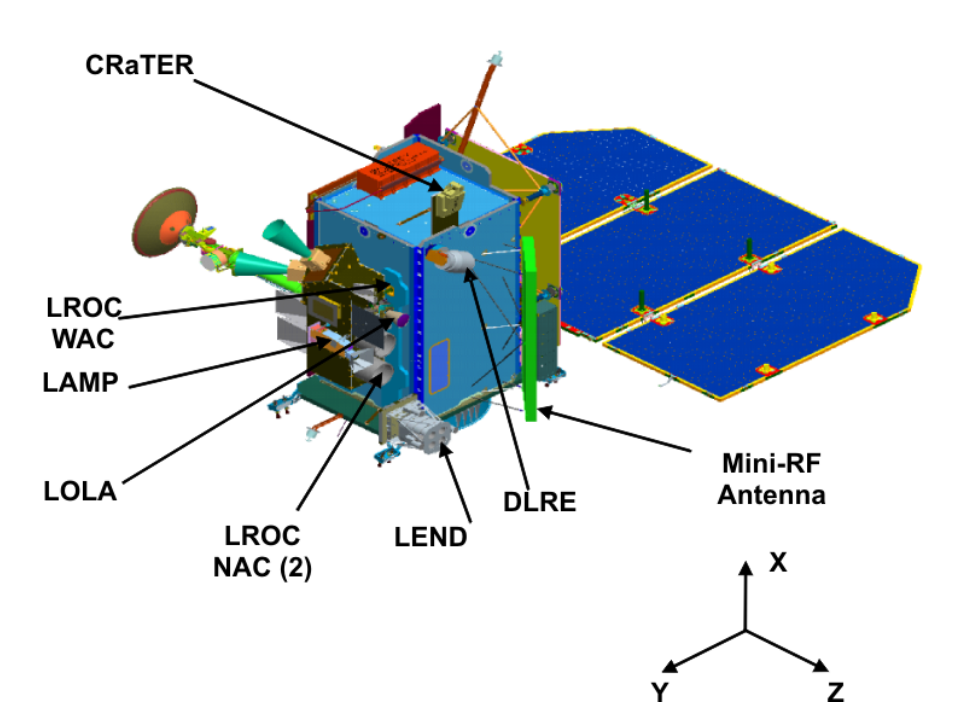
\includegraphics[width=\textwidth]{LROC-schema.png}
        \caption{Schematic of LRO with labeled instruments, showcasing its advanced suite for lunar exploration.}
        \label{fig:lro_schema}
    \end{minipage}
\end{figure}

\subsection*{LRO Instrument Suite}
The LRO is equipped with six key instruments and one technology demonstration unit, each designed to address specific scientific and exploration objectives. Table \ref{tab:lro_instruments} summarizes these instruments and their contributions:

\begin{table}[h!]
    \centering
    \caption{Summary of LRO Instruments and Their Key Contributions \cite{lro}}
    \label{tab:lro_instruments}
    \begin{tabular}{|p{3.5cm}|p{5cm}|p{4.5cm}|}
        \hline
        \textbf{Instrument} & \textbf{Primary Function} & \textbf{Significance} \\
        \hline \hline
        Lunar Orbiter Laser Altimeter: \textbf{LOLA} & Measures global topography, surface roughness, and polar illumination conditions & Identifies landing sites and potential polar ice deposits \\
        \hline
        Lunar Reconnaissance Orbiter Camera: \textbf{LROC} & Acquires high-resolution images and polar maps & Supports landing site selection and geological studies \\
        \hline
        Lunar Exploration Neutron Detector: \textbf{LEND} & Maps neutron flux to identify hydrogen-rich areas & Locates potential water-ice in lunar soil \\
        \hline
        Diviner Lunar Radiometer Experiment: \textbf{DLRE} & Maps surface temperatures and thermal environments & Identifies cold traps and ice stability regions \\
        \hline
        Lyman-Alpha Mapping Project: \textbf{LAMP} & Maps surface frost and permanently shadowed regions & Supports identification of water-ice and dark polar terrains \\
        \hline
        Cosmic Ray Telescope for the Effects of Radiation: \textbf{CRaTER} & Measures radiation effects on tissue-equivalent materials & Assesses risks for future human exploration \\
        \hline
        \textbf{Mini-RF} Technology Demonstration & Demonstrates radar imaging and interferometry & Locates potential subsurface ice deposits \\
        \hline
    \end{tabular}
\end{table}


\textbf{GRAIL (NASA):} 
The Gravity Recovery and Interior Laboratory (GRAIL) mission, comprising the twin spacecraft Ebb and Flow, mapped the Moon’s gravity field in unprecedented detail. Its data revealed mass deficits consistent with large subsurface voids, including potential lava tubes \cite{GRAIL}.

\begin{figure}[H]
    \centering
    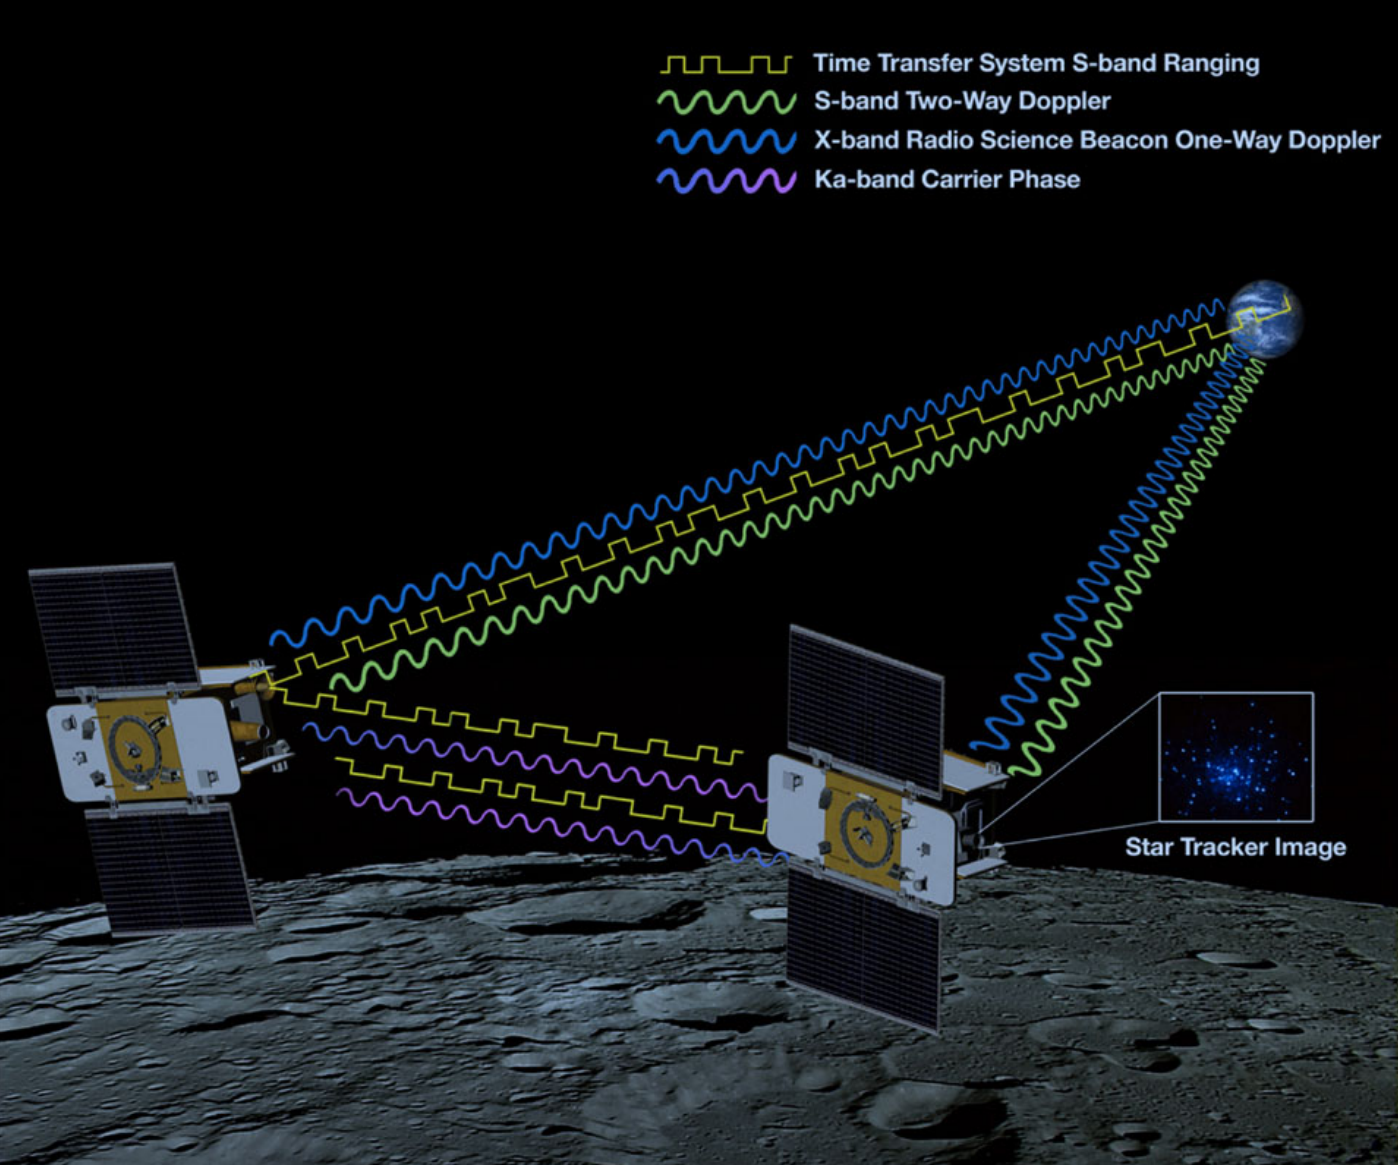
\includegraphics[width=0.52\linewidth]{grail.png}
    \caption{A render of the GRAIL mission satellites used to measure gravity gradients of the Moon \cite{GRAIL}.}
    \label{fig:grail-render}
\end{figure}

\subsection{Future Planned Missions}


\textbf{Daedalus Rover (ESA):} 
The European Space Agency (ESA) is developing the \textbf{Daedalus} (Descent And Exploration in Deep Autonomy of Lunar Underground Structures) mission to autonomously explore the \textbf{Marius Hills Lunar Pit}, a skylight into one of the Moon’s most prominent lava tubes. Designed by the University of Würzburg, the spherical Daedalus probe will be lowered into the pit using a tethered system. Equipped with 3D lidar and stereo cameras, it will map the cave’s interior in unprecedented detail, analyze structural stability, and measure environmental conditions such as radiation levels and thermal stability \cite{esa-daedalus}.

\begin{figure}[H]
    \centering
    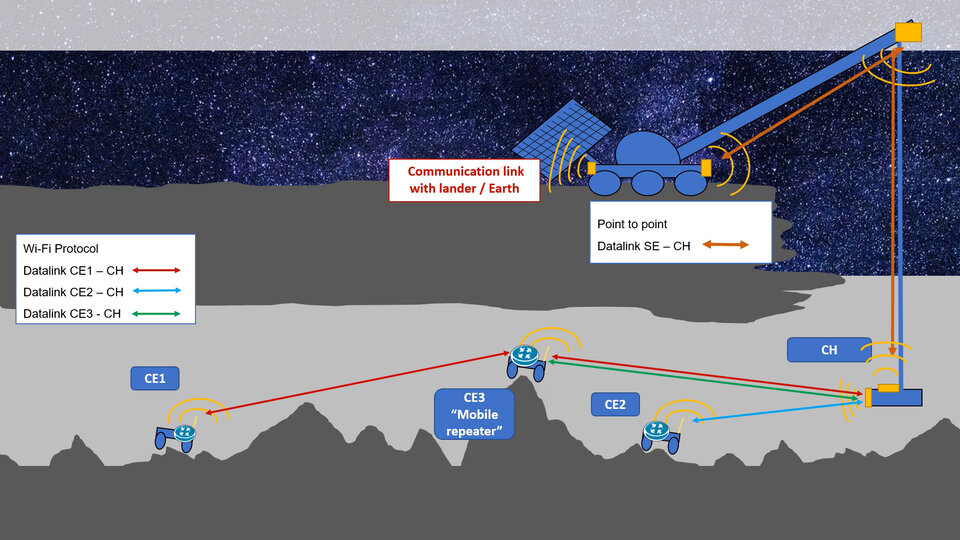
\includegraphics[width=0.8\linewidth]{daedalus-schema.png}
    \caption{Caption}
    \label{fig:daedalus-mission-schema}
\end{figure}

This mission forms part of ESA’s strategy to study lunar caves as natural shelters for future human explorers, offering protection from radiation, micrometeoroids, and extreme temperatures. Daedalus will also search for subsurface resources, such as ice or mineral deposits, that could support long-term lunar habitation. The mission is expected to operate for one lunar day (14 Earth days), using the European Large Logistics Lander (EL3) for deployment \cite{esa-daedalus}.

\begin{figure}[H]
    \centering
    \begin{minipage}[b]{0.15\textwidth}
        \centering
        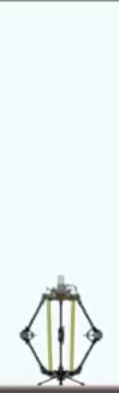
\includegraphics[width=0.82\textwidth]{daedalus-jumper-1.png}
        \caption*{Static position}
    \end{minipage}
    \hspace{0.02\textwidth}
    \begin{minipage}[b]{0.15\textwidth}
        \centering
        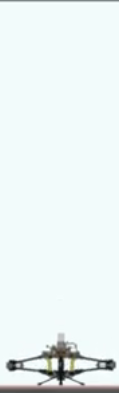
\includegraphics[width=0.82\textwidth]{daedalus-jumper-2.png}
        \caption*{Preparation to jump}
    \end{minipage}
    \hspace{0.02\textwidth}
    \begin{minipage}[b]{0.15\textwidth}
        \centering
        
\includegraphics[width=0.82\textwidth]{daedalus-jumper-3.png}
        \caption*{Mid-air jump}
    \end{minipage}
    \caption{Stages of movement for a lunar jumping robot exploring a lava tube. Each stage highlights critical aspects of its locomotion.}
    \label{fig:lunar_robot_movement}
\end{figure}


\textbf{Moon Diver Mission (NASA):} 
The Moon Diver mission is a proposed planetary exploration concept designed to utilize the Axel Extreme Terrain Rover to investigate the Tranquillitatis Pit, a 125-meter-deep lunar mare pit that reveals stratified layers of basalt deposits. This mission would provide an unprecedented opportunity to study the composition, morphology, and history of lunar mare basalts by descending into and analyzing these exposed layers \cite{kerber2023,kerber2016}.

The Axel rover, a highly specialized tethered system, is capable of rappelling into steep terrains. It construction is similar to a common rover, but it utilizes an unique mechanism of detachable forward axle, which could be secured by 300 m long tether. It is equipped with an innovative tether mechanism that not only facilitates controlled descent and ascent but also provides communication and power, which are essential for operations in permanently shadowed regions. This capability ensures that the rover can function effectively within the harsh lunar environment, even in areas devoid of sunlight \cite{kerber2016}.

The mission's scientific payload includes the Multispectral Microimager (MMI) for mineralogical analysis, an Alpha Particle X-ray Spectrometer (APXS) for chemical composition studies, and multiple cameras such as FarCam and CloseCams to document the stratigraphy of the pit walls. These instruments will allow the characterization of mare basalts, distinguishing between high-flux and low-flux lava flows and providing insights into the thermal and volcanic history of the Moon. Additionally, the rover’s onboard cameras will reconstruct 3D topographic models of the pit's interior during descent \cite{kerber2023,kerber2016}.


\begin{figure}[H]
    \centering
    \begin{minipage}[b]{0.49\textwidth}
        \centering
        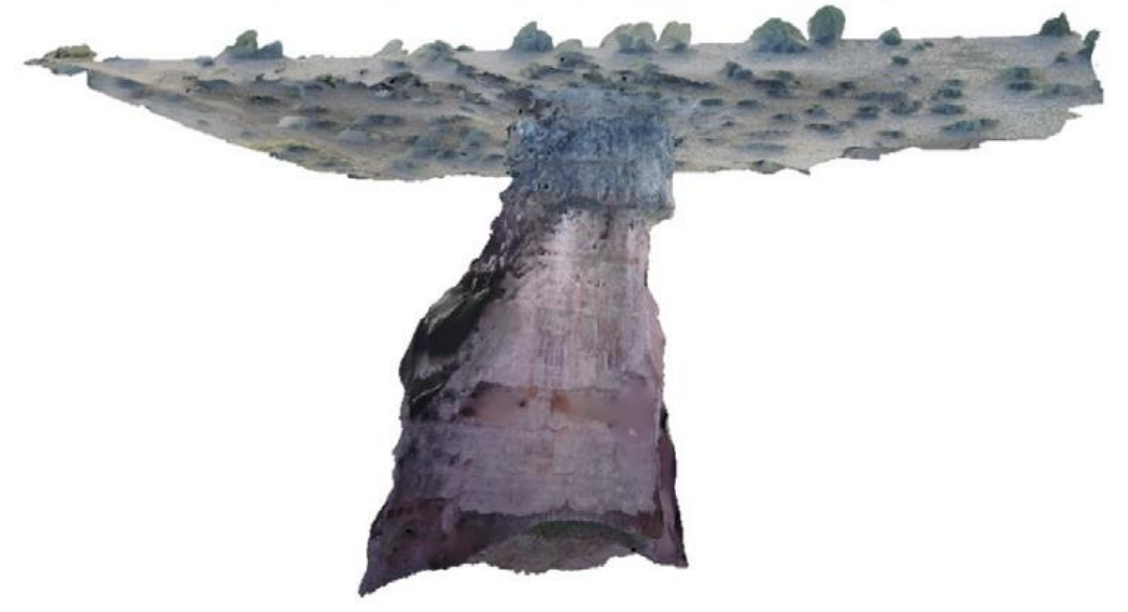
\includegraphics[width=0.82\textwidth]{moon-diver-pit-recon.png}
        \caption{3D reconstruction of a terrestrial pit, using the Moon Diver prototype \cite{kerber2023}.}
    \end{minipage}
    \begin{minipage}[b]{0.49\textwidth}
        \centering
        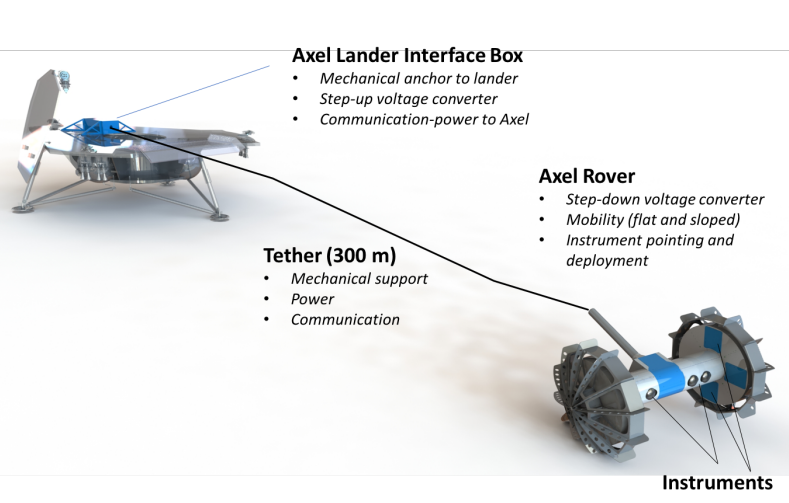
\includegraphics[width=0.82\textwidth]{moon-diver-schemoid.png}
        \caption{A schematic visualization of the robot and its parts \cite{nesnas2019}.}
    \end{minipage}
\end{figure}
